%\subsubsection{PFCA standards}
%Another source of error could be the homogeneity of the PFAS standards. If the standards were not shaken (vortexed) properly before pipetting, the PFAS solution could be unevenly dissolved and thus cause inconsistent concentrations pipetted into each centrifuge tube. This can be particularly significant for the long-chain PFCAs which are less soluble than the short-chain ones. 

%What we did to overcome this, analyzed the standards themselves and compared with calculated concentrations. 

\begin{table}
\centering
\caption{pH, conductivity, TOC and total nitrogen, cation exchange capacity (CEC) for the soil blank used in the batch tests}
\label{tab:soilsummary}
\adjustbox{max width=\textwidth}{
\begin{tabular}{llllll}
\textbf{pH ($\mathrm{H_2O}$)} & \textbf{pH (0.01 M $\mathrm{CaCl_2}$)} & \textbf{Conductivity ($\mu S/cm$)} & \textbf{TOC (\%)} & \textbf{N-tot (\%)} & CEC (meqv/100g) \\
5.38    ± 0.02    & 4.36  ± 0.01               & 23.33  ± 0.05                 & 1.32  ± 0.03      & 0.11  ± 0.003    & 2.62 ± 0.07  
\end{tabular}}
\end{table}

\begin{table}
\centering
\caption{Surface area and pore volume for the biochars produced for the batch tests.}
\adjustbox{max width=\textwidth}{
\label{tab:SAPV}
\begin{tabular}{llllll}
\toprule
Biochar  &  Pyrolysis  & \multicolumn{2}{c}{N\textsubscript{2} sorption} & \multicolumn{2}{c}{CO\textsubscript{2} sorption} \\  
         sorbent     &  temperature & \multicolumn{2}{c}{(pores \textgreater 1.5 nm)} & \multicolumn{2}{c}{(pores 0.4-1.5 nm)}\\ \cmidrule(l){3-4} \cmidrule(l){5-6}
              & (\textdegree C) & Surface area         & Pore volume         & Surface area          & Pore volume         \\
 &  & $\mathrm{m^2~g^{-1}}$  & cm\textsuperscript{3} g\textsuperscript{-1}           & $\mathrm{m^2~g^{-1}}$            & cm\textsuperscript{3} g\textsuperscript{-1}           \\ \midrule
ULS         & 700                    & 128         & 0.126          & 164.58          & 0.047          \\
CWC         & 700                    & 323         & 0.017          & 683.27          & 0.186          \\
DSL         & 700                    & 110         & 0.111          & 86.55           & 0.027         \\ \midrule
\end{tabular}}
\end{table}

\begin{table}
\caption{Effective cross-sectional diameter (D\textsubscript{eff}) and maximum diameter (D\textsubscript{max}) of TCs interpolated and extrapolated by linear regression from calculations performed by \citep{inoue2012size} on PFOA and other PFCAs with chain lengths 11-18.}
\centering
\begin{threeparttable}
\label{tab:molecsize}
\begin{tabular}{lcll}
\toprule
Compound & \begin{tabular}[l]{@{}l@{}}Carbon chain \\ length\end{tabular} & \begin{tabular}[c]{@{}l@{}}D\textsubscript{eff} \\ (nm)\end{tabular} & \begin{tabular}[c]{@{}l@{}}D\textsubscript{max} \\ (nm)\end{tabular} \\ \midrule
PFPeA    & 5                                                              & 0.45                                                 & 0.96                                                 \\
PFHxA    & 6                                                              & 0.50                                                 & 1.08                                                 \\
PFHpA    & 7                                                              & 0.56                                                 & 1.19                                                 \\
PFOA\textsuperscript{*}     & 8                                                              & 0.61                                                 & 1.36                                                 \\
PFNA     & 9                                                              & 0.67                                                 & 1.42                                                 \\
PFDA     & 10                                                             & 0.72                                                 & 1.54  \\ \bottomrule                                    
\end{tabular}
\begin{tablenotes}
\item \textsubscript{*} Calculated value from \citep{inoue2012size}
\end{tablenotes}
\end{threeparttable}
\end{table}

\begin{table}
\caption{Freundlich sorption parameters of single TC isotherms in CWC, ULS and DSL (n=9). The error is presented as standard error. All $K_F$ data are in units of $\mathrm{(\mu g/kg)/(\mu g/L)^{n_F}}$.}
\centering
\adjustbox{max width=\textwidth}{%
\begin{threeparttable}
\label{tab:summary_stats_single}
\begin{tabular}{llllllllllll}
\toprule
\multicolumn{1}{c}{Biochar} & \multicolumn{1}{c}{Compound} & \multicolumn{3}{c}{$log~K_{F,BC}$} & \multicolumn{3}{c}{$n_{F,BC}$} & \multicolumn{3}{c}{$r^2$} & $p$ \\ \midrule
CWC                                  & PFPeA                                 & 3.98        & ±        & 0.36        & 0.56      & ±      & 0.33      & 0.30       & ±       & 0.31            & -             \\
CWC                                  & PFHxA                     & 3.01        & ±        & 0.32        & 0.69      & ±      & 0.17      & 0.68       & ±       & 0.67               & **           \\
CWC                                  & PFHpA                     & 4.44        & ±        & 0.05        & 0.59      & ±      & 0.11      & 0.80       & ±       & 0.16               & **           \\
CWC                                  & PFOA                      & 5.06        & ±        & 0.08        & 0.39      & ±      & 0.05      & 0.90       & ±       & 0.10               & ***          \\
CWC                                  & PFNA                      & 4.88        & ±        & 0.04        & 0.65      & ±      & 0.04      & 0.98       & ±       & 0.05               & ***          \\
CWC                                  & PFDA                      & 5.22        & ±        & 0.07        & 0.45      & ±      & 0.04      & 0.94       & ±       & 0.08               & ***          \\
DSL                                  & PFPeA                     & 4.25        & ±        & 0.74        & 0.14      & ±      & 0.38      & 0.06       & ±       & 0.07               & -             \\
DSL                                  & PFHxA                     & 3.16        & ±        & 0.04        & 1.22      & ±      & 0.03      & 1.00       & ±       & 0.09               & ***          \\
DSL                                  & PFHpA                     & 4.67        & ±        & 0.06        & 0.57      & ±      & 0.09      & 0.86       & ±       & 0.13               & ***          \\
DSL                                  & PFOA                      & 5.12        & ±        & 0.02        & 0.60      & ±      & 0.02      & 0.99       & ±       & 0.03               & ***          \\
DSL                                  & PFNA                      & 5.33        & ±        & 0.03        & 0.80      & ±      & 0.07      & 0.94       & ±       & 0.08               & ***          \\
DSL                                  & PFDA                      & 5.61        & ±        & 0.02        & 0.61      & ±      & 0.02      & 0.99       & ±       & 0.03               & ***          \\
ULS                                  & PFPeA                     & 4.10        & ±        & 0.13        & 0.67      & ±      & 0.16      & 0.74       & ±       & 0.17               & **           \\
ULS                                  & PFHxA                     & 4.80        & ±        & 0.06        & 0.34      & ±      & 0.09      & 0.72       & ±       & 0.13               & **           \\
ULS                                  & PFHpA                     & 5.98        & ±        & 0.17        & 1.08      & ±      & 0.11      & 0.93       & ±       & 0.10               & ***          \\
ULS                                  & PFOA                      & 5.73        & ±        & 0.02        & 0.65      & ±      & 0.05      & 0.95       & ±       & 0.07               & ***          \\
ULS                                  & PFNA                      & 5.89        & ±        & 0.02        & 0.71      & ±      & 0.03      & 0.99       & ±       & 0.04               & ***          \\
ULS                                  & PFDA                      & 6.00        & ±        & 0.04        & 0.35      & ±      & 0.05      & 0.86       & ±       & 0.13               & ***     \\ \bottomrule    
\end{tabular}
\begin{tablenotes}
\item Significant codes: *** $\sim$ 0.001, ** $\sim$ 0.01, - $>$ 0.05 
\end{tablenotes}
\end{threeparttable}}
\end{table}

\begin{figure}
    \centering
    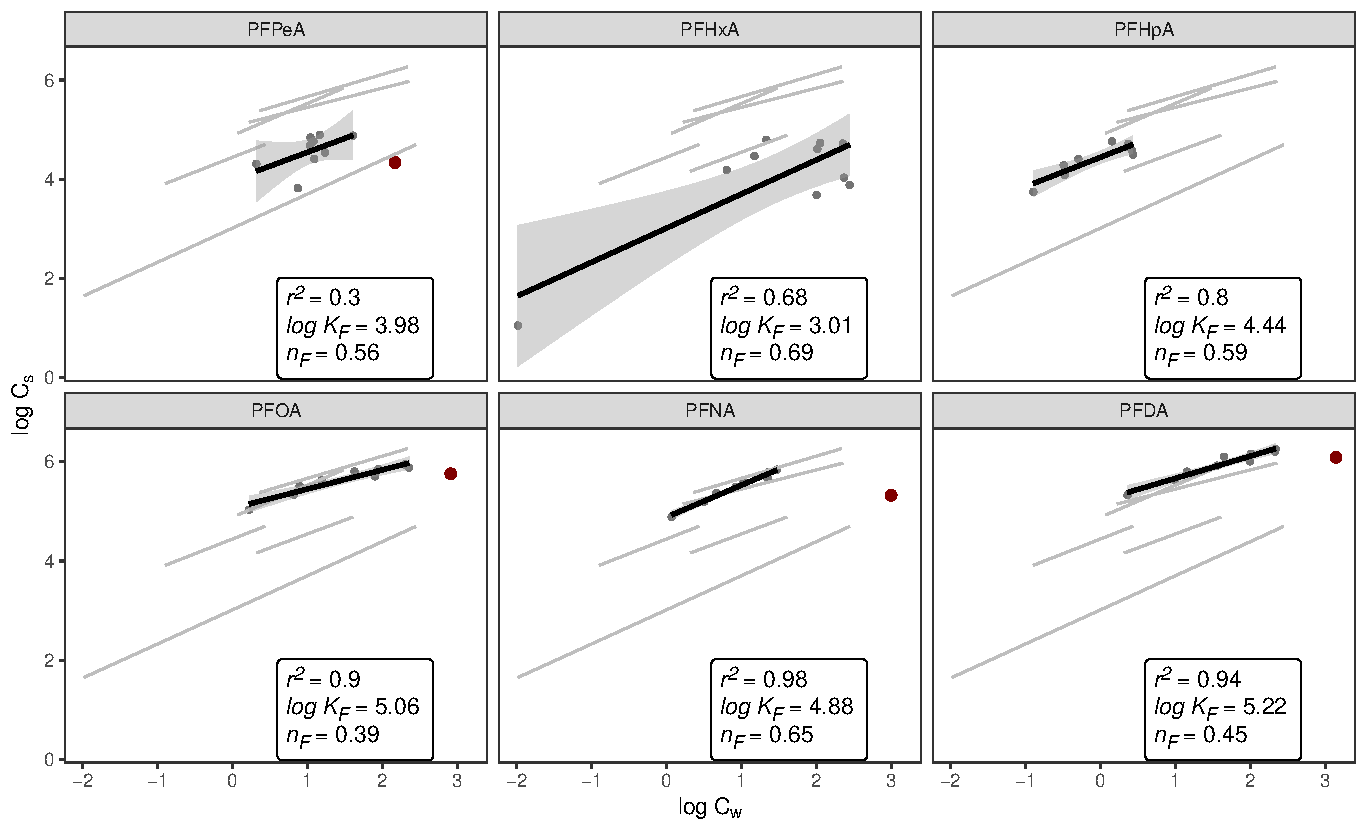
\includegraphics[width=\textwidth]{R/figs/CWC_facet_isotherm.pdf}
    \caption{Freundlich isotherms of TCs in CWC batch tests. Lines are obtained by linear regression.}
    \label{fig:CWC_isotherm2}
\end{figure}

\begin{figure}
    \centering
    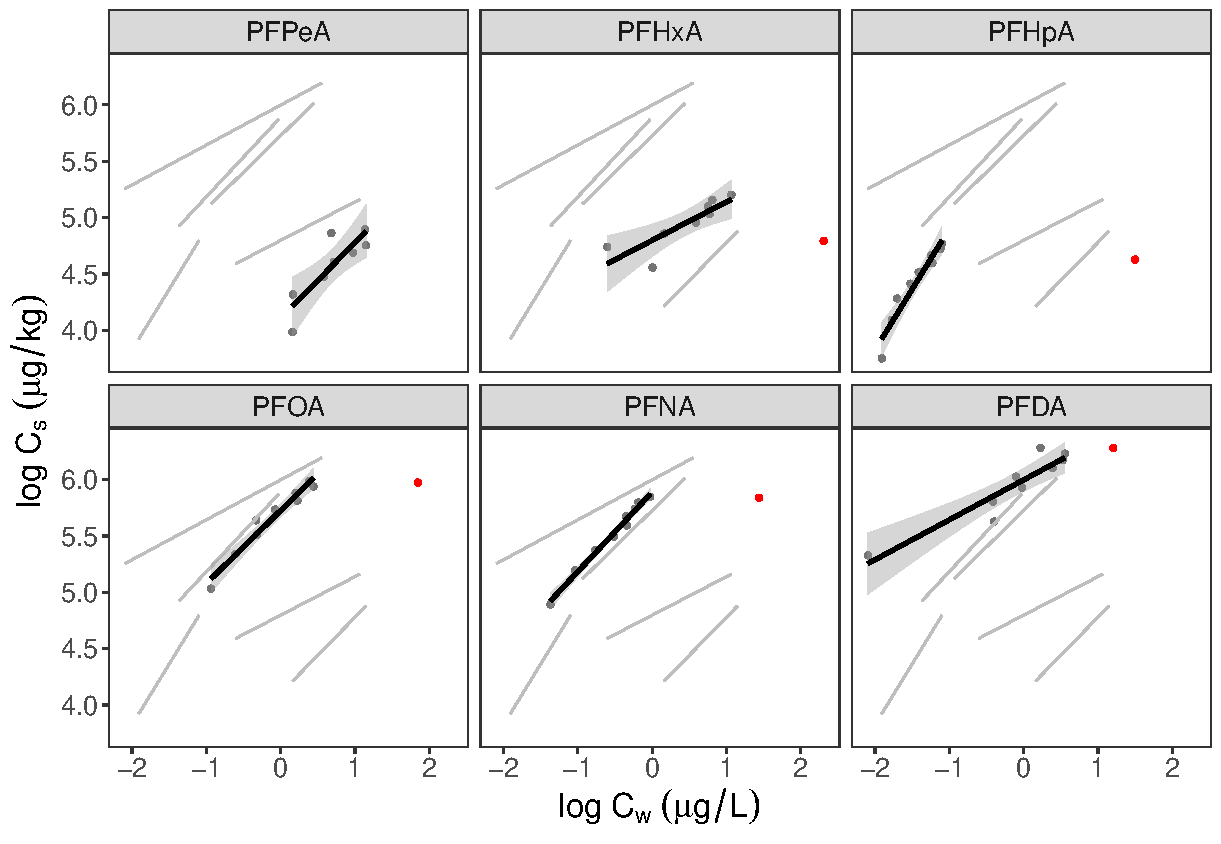
\includegraphics[width=\textwidth]{R/figs/ULS_facet_isotherm.pdf}
    \caption{Freundlich isotherms of TCs in ULS batch tests. Lines are obtained by linear regression.}
    \label{fig:ULS_isotherm2}
\end{figure}

\begin{figure}
    \centering
    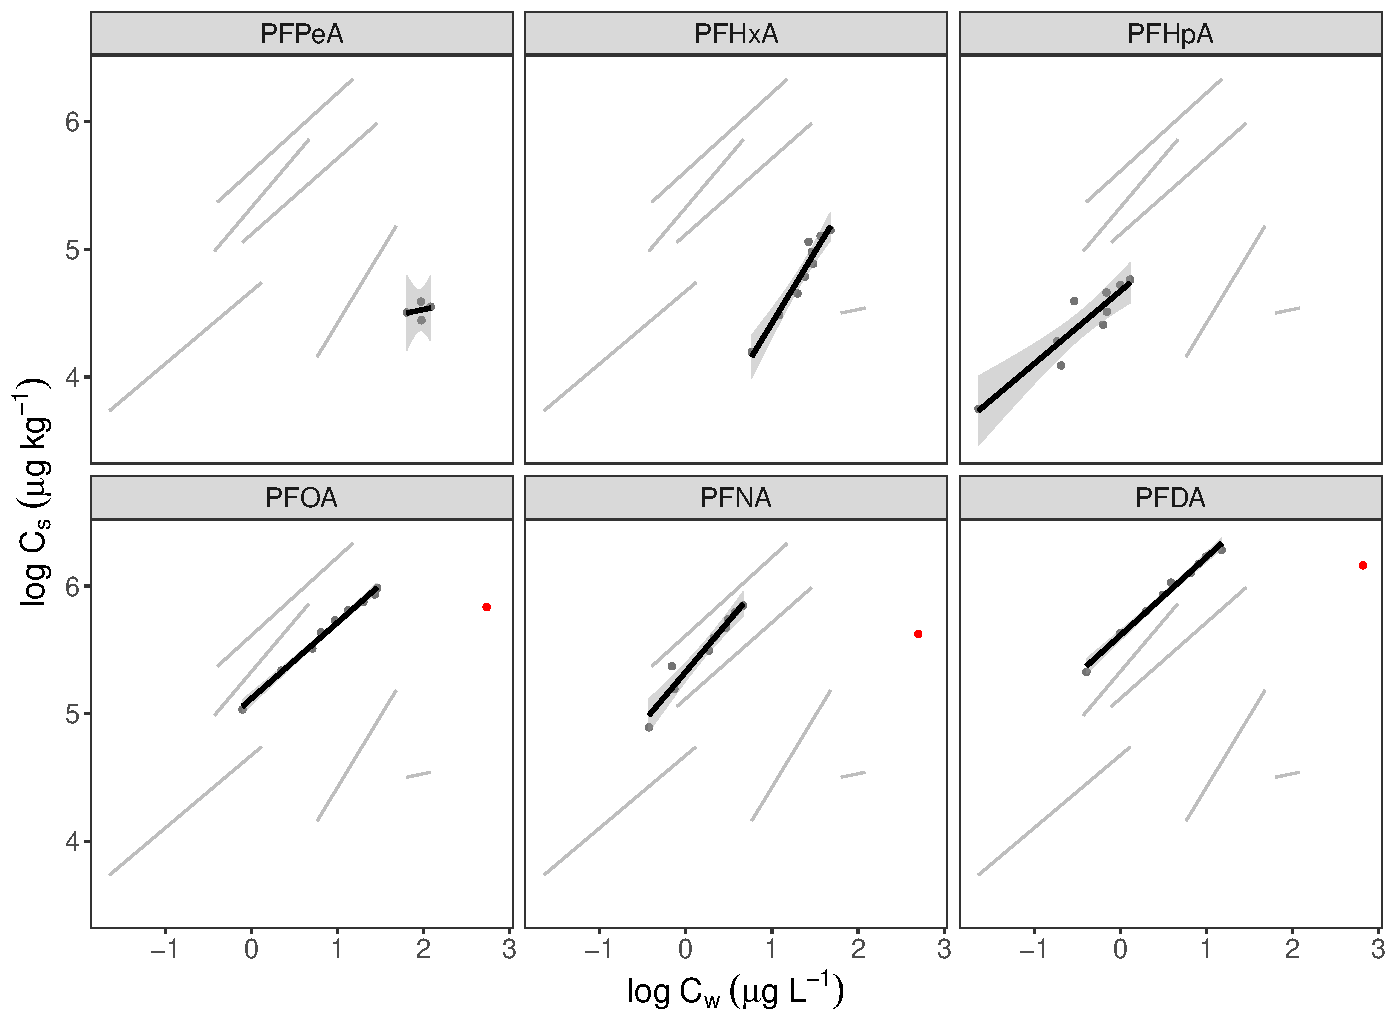
\includegraphics[width=\textwidth]{R/figs/DSL_facet_isotherm.pdf}
    \caption{Freundlich isotherms of TCs in DSL batch tests. Lines are obtained by linear regression.}
    \label{fig:DSL_isotherm2}
\end{figure}
